%% FullCourse_10Lecs -- Lecture 4, Topic 4.3: Euler Equation Method + PyTorch
%% Source: ./archive_pre_split/Lec04_DL_RL_Macro.tex (sections 5-6)
%% Pass B: layer in refinements from
%%         ../../MiniCourse_8hr/Slides/Module2_DL_RL_Macro/M2_T2_Euler_DL.tex

%% Shared preamble for the FullCourse_10Lecs topic decks.
%%
%% Each topic .tex \input's this file, then defines its own \title, \date
%% override (if any), \graphicspath, and \begin{document}.
%%
%% Reconstructed verbatim from the inlined copy preserved in
%% Lec10_Case_Studies/Lec10_T8_Case6_DeepRamsey.tex (lines 23-190), which is
%% explicitly annotated there as "from ../shared_preamble.tex, copied verbatim".
%% Base preamble matches MiniCourse_8hr/Slides/shared_preamble.tex; this version
%% additionally provides \sectiondivider, the conceptbox/cautionbox/examplebox/
%% takeawaybox tcolorboxes, and \compacttables used across the split decks.

\documentclass[10pt,english,aspectratio=169]{beamer}

\usepackage{ae,aecompl}
\usepackage[T1]{fontenc}
\usepackage{textcomp}
\usepackage[utf8]{inputenc}
\usepackage{babel}
\usepackage{datetime2}

\setcounter{secnumdepth}{3}
\setcounter{tocdepth}{3}

\usepackage{amsmath, amssymb, amsthm, graphicx}
\usepackage{booktabs, multirow}
\usepackage{tikz}
\usepackage{pgfplots}
\pgfplotsset{compat=1.16}
\usepackage[most]{tcolorbox}
\tcbuselibrary{skins, breakable, theorems}
\usepackage{listings}
\usepackage{xcolor}

\lstset{
  basicstyle=\ttfamily\small,
  keywordstyle=\color{blue!80!black}\bfseries,
  commentstyle=\color{green!50!black}\itshape,
  stringstyle=\color{orange!80!black},
  backgroundcolor=\color{gray!8},
  frame=single,
  rulecolor=\color{gray!40},
  breaklines=true,
  showstringspaces=false,
  numbers=none,
}

\lstdefinestyle{pythonstyle}{
    language=Python,
    basicstyle=\ttfamily\footnotesize,
    keywordstyle=\color{blue!80!black}\bfseries,
    commentstyle=\color{green!50!black}\itshape,
    stringstyle=\color{orange!80!black},
    frame=single,
    breaklines=true,
    showstringspaces=false,
    numbers=left,
    numbersep=5pt,
    numberstyle=\tiny\color{gray},
    backgroundcolor=\color{gray!8},
    rulecolor=\color{gray!40}
}

\ifx\hypersetup\undefined
  \AtBeginDocument{%
    \hypersetup{bookmarks=false,breaklinks=true,pdfborder={0 0 0},colorlinks=true,
      linkcolor=DarkText,urlcolor=RedTitle}%
  }
\else
  \hypersetup{bookmarks=false,breaklinks=true,pdfborder={0 0 0},colorlinks=true,
    linkcolor=DarkText,urlcolor=RedTitle}%
\fi

\makeatletter
\newcommand\makebeamertitle{%
  \begin{frame}[plain]
    \vspace*{1.0cm}
    \centering
    {\usebeamerfont{title}\usebeamercolor[fg]{title}\inserttitle\par}
    \vspace{1.0cm}
    {\usebeamerfont{author}\usebeamercolor[fg]{author}\insertauthor\par}
    \vspace{0.2cm}
    {\usebeamerfont{date}\usebeamercolor[fg]{date}\insertdate\par}
  \end{frame}}%
\AtBeginDocument{%
  \let\origtableofcontents=\tableofcontents
  \def\tableofcontents{\@ifnextchar[{\origtableofcontents}{\gobbletableofcontents}}
  \def\gobbletableofcontents#1{\origtableofcontents}%
}

\usetheme{metropolis}
\usefonttheme{professionalfonts}

\definecolor{LightGray}{RGB}{230,230,230}
\definecolor{RedTitle}{RGB}{0,0,200}
\definecolor{VeryLightGray}{RGB}{245,245,245}
\definecolor{DarkText}{RGB}{0,0,0}

\setbeamercolor{background canvas}{bg=white}
\setbeamercolor{title}{fg=RedTitle}
\setbeamercolor{author}{fg=DarkText}
\setbeamercolor{date}{fg=DarkText}
\setbeamercolor{frametitle}{bg=VeryLightGray,fg=DarkText}
\setbeamercolor{normal text}{fg=DarkText}
\setbeamerfont{title}{size=\large}

\setbeamersize{text margin left=5mm, text margin right=5mm}
\addtobeamertemplate{frametitle}{}{\vspace{-0.5em}}
\newcommand{\reducevspace}{\vspace{-0.5cm}}

% Shared section divider and box styles for split topic decks.
\newcommand{\sectiondivider}[2]{%
\begin{frame}[plain,noframenumbering]
\begin{center}
\vfill
{\Large\textbf{#1}\par}
\vspace{0.35cm}
{\normalsize #2\par}
\vfill
\end{center}
\end{frame}
}

\newtcolorbox{conceptbox}[1][]{
  colback=blue!3,
  colframe=RedTitle!55,
  boxrule=0.35mm,
  arc=1mm,
  left=2mm,
  right=2mm,
  top=1mm,
  bottom=1mm,
  #1
}
\newtcolorbox{cautionbox}[1][]{
  colback=red!3,
  colframe=red!50!black,
  boxrule=0.35mm,
  arc=1mm,
  left=2mm,
  right=2mm,
  top=1mm,
  bottom=1mm,
  #1
}
\newtcolorbox{examplebox}[1][]{
  colback=green!3,
  colframe=green!45!black,
  boxrule=0.35mm,
  arc=1mm,
  left=2mm,
  right=2mm,
  top=1mm,
  bottom=1mm,
  #1
}
\newtcolorbox{takeawaybox}[1][]{
  colback=VeryLightGray,
  colframe=RedTitle!55,
  boxrule=0.35mm,
  arc=1mm,
  left=2mm,
  right=2mm,
  top=1mm,
  bottom=1mm,
  #1
}
\newcommand{\compacttables}{\renewcommand{\arraystretch}{1.15}}

\setbeamertemplate{navigation symbols}{}
\setbeamertemplate{footline}{%
  \hfill%
  \usebeamercolor[fg]{page number in head/foot}%
  \usebeamerfont{page number in head/foot}%
  \insertframenumber\,/\,\inserttotalframenumber\kern1em\vskip2pt%
}

\makeatother

\author{Zhigang Feng}
% "date with time": compile timestamp so each build is identifiable.
\date{\today\ \DTMcurrenttime}


\graphicspath{{./pic/}{../../MiniCourse_8hr/Slides/Module2_DL_RL_Macro/pic/}{../}}

% Suppress the redundant auto-generated metropolis section page; the
% \sectiondivider frames below are the dividers we keep.
\metroset{sectionpage=none}
\usetikzlibrary{positioning,arrows.meta,shapes,calc}
%% Lec04 shared MAP slide: "one map, four acts" recurring diagram.
%% Input this file AFTER ../shared_preamble.tex (needs RedTitle, VeryLightGray,
%% DarkText) and AFTER \usetikzlibrary{positioning,arrows.meta,shapes,calc}.
%% Call \LecFourMap{k} inside a frame, where k in {1,2,3,4} highlights the
%% current act ("you are here") and k = 0 renders the closing reprise with all
%% four acts checked green (used by T4's closing frame).
%% Filename deliberately does NOT match the build glob Lec*_T*.tex, so the build
%% script never tries to compile it standalone.
%%
%% The four acts are the lecture's story: PROBLEM -> SOLVE -> CODE -> TRUST,
%% one running example throughout (the optimal growth model): why grids break,
%% the Bellman route (deep VFI + actor-critic), the Euler route in PyTorch,
%% and structured networks + the validation gate.

\newcommand{\LecFourMap}[1]{%
% Precompute per-box style selectors; TikZ option lists are comma-split before
% TeX conditionals run, so \ifnum must not sit inside a [...] options list.
\ifnum#1=0
  \tikzset{lmapa/.style={lmapdone}, lmapb/.style={lmapdone},
           lmapc/.style={lmapdone}, lmapd/.style={lmapdone}}%
\else
  \tikzset{lmapa/.style={}, lmapb/.style={}, lmapc/.style={}, lmapd/.style={}}%
  \ifnum#1=1 \tikzset{lmapa/.style={lmapcur}}\fi
  \ifnum#1=2 \tikzset{lmapb/.style={lmapcur}}\fi
  \ifnum#1=3 \tikzset{lmapc/.style={lmapcur}}\fi
  \ifnum#1=4 \tikzset{lmapd/.style={lmapcur}}\fi
\fi
\begin{center}
\begin{tikzpicture}[
    act/.style={rectangle, rounded corners, draw=black!60, fill=VeryLightGray,
        minimum width=3.0cm, minimum height=0.95cm, text width=2.9cm,
        align=center, font=\small, text=DarkText},
    lmapcur/.style={draw=RedTitle, very thick, fill=orange!20},
    lmapdone/.style={draw=green!45!black, thick, fill=green!10},
    q/.style={font=\tiny\itshape, text width=3.0cm, align=center, text=black!70},
    barlab/.style={font=\tiny\bfseries, text=black!65},
    sat/.style={rectangle, rounded corners, draw=black!45, dashed, fill=white,
        text width=5.2cm, align=center, font=\tiny, text=black!70,
        minimum height=0.5cm},
    arr/.style={-{Stealth[length=2.2mm]}, thick, gray!60}
]
    % --- four act boxes ---
    \node[act, lmapa] (a1) at (0,0)
        {\textbf{4.1\ \ PROBLEM}\\[1pt] \tiny growth model $\cdot$ curse of dim.};
    \node[act, lmapb] (a2) at (3.6,0)
        {\textbf{4.2\ \ SOLVE}\\[1pt] \tiny deep VFI $\cdot$ actor--critic};
    \node[act, lmapc] (a3) at (7.2,0)
        {\textbf{4.3\ \ CODE}\\[1pt] \tiny Euler loss $\cdot$ PyTorch};
    \node[act, lmapd] (a4) at (10.8,0)
        {\textbf{4.4\ \ TRUST}\\[1pt] \tiny ICNN $\cdot$ validation $\cdot$ lab};
    \draw[arr] (a1) -- (a2);
    \draw[arr] (a2) -- (a3);
    \draw[arr] (a3) -- (a4);
    % --- the student question each act answers ---
    \node[q] at (0,-0.95)    {why do grids break on\\ real macro models?};
    \node[q] at (3.6,-0.95)  {how do neural nets solve\\ the Bellman equation?};
    \node[q] at (7.2,-0.95)  {how do I code it --- loss,\\ networks, training loop?};
    \node[q] at (10.8,-0.95) {can I trust the answer ---\\ and how do I prove it?};
    % --- "you are here" marker above the current act ---
    \ifnum#1=1 \node[font=\scriptsize\bfseries, text=RedTitle] at (0,0.98)
        {you are here\ $\blacktriangledown$};\fi
    \ifnum#1=2 \node[font=\scriptsize\bfseries, text=RedTitle] at (3.6,0.98)
        {you are here\ $\blacktriangledown$};\fi
    \ifnum#1=3 \node[font=\scriptsize\bfseries, text=RedTitle] at (7.2,0.98)
        {you are here\ $\blacktriangledown$};\fi
    \ifnum#1=4 \node[font=\scriptsize\bfseries, text=RedTitle] at (10.8,0.98)
        {you are here\ $\blacktriangledown$};\fi
    \ifnum#1=0 \node[font=\scriptsize\bfseries, text=green!45!black] at (5.4,0.98)
        {all four acts complete};\fi
    % --- bottom band: two solution routes + the audit (the technical spine) ---
    \fill[blue!10]   (-1.55,-1.72) rectangle (5.15,-1.40);
    \fill[green!12]  (5.65,-1.72)  rectangle (8.75,-1.40);
    \fill[orange!16] (9.25,-1.72)  rectangle (12.35,-1.40);
    \node[barlab] at (1.8,-1.56)  {BELLMAN ROUTE\ ($V$, $g$ networks)};
    \node[barlab] at (7.2,-1.56)  {EULER ROUTE\ (FOC residuals)};
    \node[barlab] at (10.8,-1.56) {AUDIT GATE\ (Lab 3A/3B)};
    % --- dashed satellites: where this lecture sits in the course flow ---
    \node[sat] at (1.5,-2.42)
        {\textit{upstream:} Lec03 --- the NN toolkit (architecture, UAT, training, ICNN)};
    \node[sat] at (9.3,-2.42)
        {\textit{downstream:} Lec05 --- the RL theory behind actor--critic; Lec06 --- heterogeneous agents at scale};
\end{tikzpicture}
\end{center}
}


\title[AI for Econ Research]{AI for Economic Research: Dynamic Models, Language, and Agents\\
Lecture 4.3: Euler-Equation Method \& PyTorch Implementation}

\begin{document}

\makebeamertitle

%=============================================================================
\begin{frame}{Lecture 4 in One Map}
\textbf{One lecture, four decks, one running example: solve the optimal growth model with deep learning --- pose the problem, solve it two ways, code it, and prove the answer right.}

\LecFourMap{3}

\vspace{0.05cm}
\footnotesize\textit{\textbf{Act 4.3 (here)} solves it the Euler way and writes the code: first-order conditions become the loss, PyTorch's autograd does the calculus, and PolicyNet/ValueNet train to the analytical solution (Lab 3B).}
\end{frame}

%=============================================================================
\section{Euler Equation Method + Supervised Learning}

\sectiondivider{Euler Equation Method + Supervised Learning}{First-order conditions as a loss function: solve by minimizing residuals}

%---------------------------------------
\begin{frame}{Context: Two Approaches to the Same Problem}
\begin{itemize}
  \item We have seen the \textbf{actor-critic} approach: train two networks to satisfy the Bellman equation
  \medskip
  \item Now we consider an alternative: \textbf{Euler equation minimization}
    \begin{itemize}
      \item Derive the first-order conditions (Euler equations)
      \item Train a \emph{single} policy network to satisfy them
    \end{itemize}
  \medskip
  \item \textbf{Comparison}:
    \begin{itemize}
      \item Actor-Critic (Bellman): Two networks, no need to derive FOCs, RL flavor
      \item Euler Equation: One network, requires deriving FOCs, supervised learning flavor
    \end{itemize}
  \medskip
  \item Both are valid; which is better depends on the model:
    \begin{itemize}
      \item Euler equation method is very precise when FOCs are available
      \item Actor-Critic is more general (handles kinks, discrete choices)
    \end{itemize}
\end{itemize}

\vspace{0.15cm}
{\footnotesize\textit{Euler-equation training is a \textbf{supervised} problem (regress the FOC residual against zero); actor-critic is \textbf{reinforcement} (policy gradient on the Bellman objective). Lec05 T3 formalizes the actor-critic loss derivation; here we treat both as PyTorch optimization.}}
\end{frame}

%---------------------------------------
\begin{frame}{The Euler Equation: Optimality Condition}
\begin{itemize}
  \item Capital accumulation: $k' = g(k)$, \quad consumption: $c = f(k) + (1-\delta)k - g(k)$
  \medskip
  \item For CRRA utility $u(c) = \frac{c^{1-\sigma}}{1-\sigma}$ and Cobb-Douglas production, the equilibrium satisfies:
    \[
      u'(c) = \beta\, u'(c')\, \bigl[\alpha\, g(k)^{\alpha-1} + 1 - \delta\bigr]
      \tag{EE}
    \]
  \medskip
  \item \textbf{Interpretation}: The marginal cost of saving today equals the discounted marginal benefit tomorrow
  \medskip
  \item \textbf{Goal}: Learn a policy $g$ that makes the \textbf{Euler residual} vanish:
    \[
      \mathcal{R}(k; g) = u'(c) - \beta\, u'(c')\bigl[\alpha\, g(k)^{\alpha-1} + 1 - \delta\bigr]
    \]
    for all economically relevant $k$
\end{itemize}
\end{frame}

%---------------------------------------
\begin{frame}{Euler Equation: Necessary but Not Sufficient}
\begin{itemize}
  \item \textbf{Important caveat}: The Euler equation is a \emph{necessary} condition for optimality, but \textbf{not sufficient} by itself
  \medskip
  \item For a complete characterization, we also need:
    \begin{itemize}
      \item \textbf{Transversality condition}: $\lim_{t\to\infty} \beta^t u'(c_t)\, k_{t+1} = 0$
      \item \textbf{Feasibility constraints}: $c \geq 0$, $k' \geq 0$
    \end{itemize}
  \medskip
  \item \textbf{Handling inequality constraints}:
    \begin{itemize}
      \item Kuhn-Tucker complementary slackness conditions arise
      \item Can be converted to equalities via Fischer-Burmeister functions or penalty methods
      \item Or handled via architectural constraints (sigmoid output)
    \end{itemize}
  \medskip
  \item For now, we focus on \textbf{interior solutions} where the Euler equation holds with equality throughout
\end{itemize}
\end{frame}

%---------------------------------------
\begin{frame}{From Euler Residual to Loss Function}
\begin{itemize}
  \item Approximate the policy by a neural network: $g(k) \approx \Gamma_{\gamma_g}(k)$
  \medskip
  \item Sample $k_i \sim D(k)$ (e.g., stationary distribution or uniform)
  \medskip
  \item Define the \textbf{mean-squared Euler residual} loss as an expectation over the sampling distribution:
    \[
      \mathcal{L}_g(\gamma_g) = \mathbb{E}_{k\sim D(k)}\bigl[\mathcal{R}(k; \Gamma_{\gamma_g})^2\bigr] \;\approx\; \frac{1}{N}\sum_{i=1}^{N} \bigl[\mathcal{R}(k_i; \Gamma_{\gamma_g})\bigr]^2
    \]
    {\footnotesize The empirical mean $\tfrac1N\sum_i$ is the special case of $\mathbb{E}_{k\sim D(k)}$ using $N$ i.i.d.\ draws.}
  \medskip
  \item \textbf{This is supervised learning}: the ``label'' for each state $k_i$ is zero (the Euler equation should hold exactly)
  \medskip
  \item Optimal policy parameters satisfy: $\nabla_{\gamma_g}\, \mathcal{L}_g(\gamma_g^*) = 0$
  \item All derivatives computed automatically via \texttt{autograd}
\end{itemize}
\end{frame}

%---------------------------------------
\begin{frame}{The Mean Value Intuition}
\begin{itemize}
  \item We minimize the \emph{average} Euler residual across sampled states:
    \[
      \mathcal{L}_g(\gamma_g) = \mathbb{E}_{k \sim D(k)}\bigl[\mathcal{R}(k; \Gamma_{\gamma_g})^2\bigr] \approx \frac{1}{N}\sum_{i=1}^{N} \mathcal{R}(k_i; \Gamma_{\gamma_g})^2
    \]
  \medskip
  \item \textbf{Intuition}:
    \begin{itemize}
      \item If a candidate policy satisfies the Euler equation \emph{on average} across all sampled states, it should be a good approximation to the true equilibrium policy
      \item If the average residual is large, the policy must be violating optimality somewhere
    \end{itemize}
  \medskip
  \item This ``average fitness'' criterion:
    \begin{itemize}
      \item Ensures global accuracy across the domain
      \item Is computationally tractable via Monte Carlo sampling
      \item Naturally integrates with gradient-based NN training
    \end{itemize}
\end{itemize}
\end{frame}

%---------------------------------------
\begin{frame}{The Stochastic Case: Expectation in the Euler Equation}
\begin{itemize}
  \item With a productivity shock $z$, the Euler equation carries a \textbf{conditional expectation} over next period's shock $z'$:
    \[
      u'(c_t) = \beta\, \mathbb{E}_{z' \mid z}\!\bigl[u'(c_{t+1})(\alpha k_{t+1}^{\alpha-1} z_{t+1} + 1 - \delta)\bigr]
    \]
  \medskip
  \item The residual $\mathcal{R}$ now depends on that inner expectation --- there is no closed form.
  \medskip
  \item \textbf{Monte-Carlo estimate}: replace $\mathbb{E}_{z'\mid z}$ by an average over $J$ shock draws $z'_{ij}$:
    \[
      \widehat{\mathcal{R}}(k_i; g) = u'(c_i) - \frac{\beta}{J}\sum_{j=1}^{J} u'(c'_{ij})\bigl[\alpha k'^{\alpha-1}_{i} z'_{ij} + 1 - \delta\bigr]
    \]
  \medskip
  \item \textbf{Two layers of sampling}: an \emph{outer} average over states $k_i\sim D(k)$ (the loss $\mathbb{E}_{k\sim D(k)}$) and an \emph{inner} average over shocks $z'_{ij}$ (this conditional expectation).
\end{itemize}
\end{frame}

%---------------------------------------
\begin{frame}{Variance Reduction: Gauss--Hermite Quadrature}
\small
\begin{itemize}
  \item Plain Monte-Carlo over $J$ random shock draws is \emph{noisy}: its error falls only like $1/\sqrt{J}$, and that noise enters every gradient.
  \medskip
  \item \textbf{Gauss--Hermite quadrature} replaces the random draws with a few \emph{deterministic} nodes $z'_j$ and weights $w_j$:
    \[
      \mathbb{E}_{z'\mid z}[h(z')] = \int h(z')\,\phi(z')\,dz' \;\approx\; \sum_{j=1}^{J} w_j\, h(z'_j),
    \]
    \emph{exact} whenever $h$ is a polynomial of degree $\le 2J-1$ (against the Gaussian weight $\phi$).
    \begin{itemize}\footnotesize
      \item Log-normal shocks $z'=e^{\mu+\sigma\varepsilon}$, $\varepsilon\sim\mathcal N(0,1)$: change variables to the standard Gaussian, then read nodes/weights from a table.
      \item \textbf{Why it works}: smooth integrands are nearly polynomial, so a handful of well-placed nodes ($J\approx 5$--$7$) match thousands of random draws --- same accuracy, \emph{zero} sampling noise.
    \end{itemize}
  \medskip
  \item \textbf{Why the loss stays differentiable}: the nodes and weights are \emph{constants}, so the loss is a fixed weighted sum of smooth network outputs --- \texttt{autograd} differentiates straight through. Mini-batching over states only changes \emph{which} states enter the sum; it never breaks the gradient (we sample exogenous shocks/states, not policy-dependent randomness, so no reparameterization trick is needed).
\end{itemize}
\end{frame}

%---------------------------------------
\begin{frame}{Neural Network for the Policy Function}
\begin{itemize}
  \item Two-hidden-layer MLP (64--64--1) with ReLU and Sigmoid:
\end{itemize}
\[
  \boxed{
    \Gamma_{\gamma_g}(k) = \sigma_2\Bigl(W_2 \cdot \sigma_1(W_1 k + b_1) + b_2\Bigr)
  }
\]
\begin{itemize}
  \item Hidden activation $\sigma_1$ = \texttt{ReLU}; output activation $\sigma_2$ = \texttt{Sigmoid}
  \item Sigmoid output is scaled to $[0, f(k) + (1-\delta)k - \varepsilon]$ to ensure feasibility:
    \[
      0 \leq \Gamma_{\gamma_g}(k) \leq f(k) + (1-\delta)k
    \]
  \medskip
  \item All derivatives $\partial \mathcal{L}_g / \partial \gamma_g$ are computed automatically by \texttt{autograd}
  \item No need to derive or code analytical Jacobians
\end{itemize}
\end{frame}

%---------------------------------------
\begin{frame}{Feasibility by Construction}
\begin{itemize}
  \item \textbf{Why Sigmoid, then rescale?}
    \begin{itemize}
      \item Sigmoid output $s \in (0,1)$ ensures $g(k) = s \cdot [f(k) + (1-\delta)k - \varepsilon]$ stays in the feasible interior
      \item Avoids generating samples with $c \leq 0$ during training (which would blow up $u'(c) = c^{-\sigma}$)
    \end{itemize}
  \medskip
  \item \textbf{Why subtract $\varepsilon$?} A small slack prevents marginal-utility divergence near $c = 0$
  \medskip
  \item \textbf{Alternatives}:
    \begin{itemize}
      \item \texttt{Softplus} output: always positive, smooth
      \item Hard \texttt{torch.clamp}: simple but kills gradients at the boundary
      \item Log-parameterization: train on $\log c$ rather than $c$
    \end{itemize}
  \medskip
  \item Architectural feasibility outperforms post-hoc clipping --- Lab 3B verifies this empirically
\end{itemize}
\end{frame}

%---------------------------------------
\begin{frame}{Minimising the Euler Residual: Training Loop}
\begin{itemize}
  \item Initialize $\gamma_g^{(0)}$; choose learning rate $\alpha_g$
  \medskip
  \item \textbf{Repeat until convergence}:
    \begin{enumerate}
      \item Draw a mini-batch $\{k_i\}_{i=1}^{B}$
      \item Compute loss $\mathcal{L}_g(\gamma_g)$ and its gradient via back-propagation
      \item Gradient step:
        \[
          \gamma_g^{(j+1)} = \gamma_g^{(j)} - \alpha_g\, \nabla_{\gamma_g} \mathcal{L}_g(\gamma_g^{(j)})
        \]
      \item Optionally resample $k_i$ from the same distribution $D(k)$
    \end{enumerate}
  \medskip
  \item \textbf{Pros of Euler method}:
    \begin{itemize}
      \item Very precise policy functions; theoretically grounded
      \item Only one network to train (simpler than actor-critic)
    \end{itemize}
  \item \textbf{Cons}: Does not yield the value function $V$; requires deriving FOCs
\end{itemize}
\end{frame}

%=============================================================================
\section{PyTorch Implementation}

\sectiondivider{PyTorch Implementation}{PolicyNet, ValueNet, and the training loop --- the code behind Lab 3B}

%---------------------------------------
\begin{frame}{Implementation Overview: Two Approaches}
\begin{itemize}\footnotesize
  \item \textbf{Approach 1 --- Deep VFI (Lab 3B, Part 1)}:
    \texttt{PolicyNet} + \texttt{ValueNet}, $T$-step lookahead with soft constraints; result = $g(k)$ \emph{and} $V(k)$.
  \item \textbf{Approach 2 --- Euler Equation (Lab 3B, Part 2)}:
    Single \texttt{PolicyNetwork}; loss = mean-squared Euler residual; result = policy $g(k)$.
  \item Both validated against the analytical solution from Lab 3A.
\end{itemize}

\vspace{0.1cm}
\begin{tcolorbox}[colback=blue!3, colframe=blue!40, fontupper=\scriptsize, boxsep=2pt, top=3pt, bottom=3pt,
                   title={\scriptsize Common PyTorch skeleton (both approaches)}]
\begin{enumerate}\scriptsize
  \item \textbf{Define networks}: \texttt{PolicyNet} (Sigmoid output, feasibility-rescaled) and/or \texttt{ValueNet}.
  \item \textbf{Build loss}: Bellman MSE = $(V(k) - (u + \beta V(k')))^2$ \emph{and/or} Euler residual = $u'(c) - \beta\,\mathbb{E}[u'(c')\,(\alpha k'^{\alpha-1} z' + 1 - \delta)]$.
  \item \textbf{Train}: \texttt{AdamW} on mini-batches sampled from $D(k)$; alternate Critic/Actor steps when both nets are present.
\end{enumerate}
\end{tcolorbox}
\end{frame}

%---------------------------------------
\begin{frame}[fragile]{Network Architecture: PolicyNet and ValueNet}
\vspace{-0.25cm}
{\footnotesize\textit{Code targets PyTorch $\geq 2.3$ (2024); AdamW optimizer per Lec03 T3:225. Lab 3A/3B notebooks use matching versions.}}
\vspace{-0.1cm}
\begin{lstlisting}[style=pythonstyle,basicstyle=\ttfamily\tiny]
class ValueNet(nn.Module):
    def __init__(self, nh=64):
        super().__init__()
        self.net = nn.Sequential(
            nn.Linear(1, nh), nn.ReLU(),
            nn.Linear(nh, nh), nn.ReLU(),
            nn.Linear(nh, 1))
    def forward(self, k): return self.net(k)

class PolicyNet(nn.Module):
    def __init__(self, alpha, eps, nh=64):
        super().__init__()
        self.alpha, self.eps = alpha, eps
        self.net = nn.Sequential(
            nn.Linear(1, nh), nn.ReLU(),
            nn.Linear(nh, nh), nn.ReLU(),
            nn.Linear(nh, 1), nn.Sigmoid())  # Output in [0, 1]
    def forward(self, k):
        max_kp = torch.clamp(k**self.alpha - self.eps, 1e-9)
        return self.net(k) * max_kp  # Scale to [0, f(k)-eps]
\end{lstlisting}
\vspace{-0.3cm}
\begin{itemize}
  \item \texttt{Sigmoid} ensures $g(k) \in [0, f(k) - \varepsilon]$: feasibility by construction
  \item \texttt{ValueNet}: unconstrained output (value can be any real number)
\end{itemize}
\end{frame}

%---------------------------------------
\begin{frame}[fragile]{Policy Evaluation: Bellman MSE}
\vspace{-0.3cm}
\begin{lstlisting}[style=pythonstyle,basicstyle=\ttfamily\tiny]
def value_update_step(self):
    self.value_optimizer.zero_grad()
    # Sample batch of capital states
    k_batch = torch.rand(self.n_batch, 1, device=self.device) \
              * (self.k_max - self.k_min) + self.k_min

    v_current = self.value_net(k_batch)           # V(k)
    kp_batch  = self.policy_net(k_batch)           # k' = g(k)
    u_batch   = self.utility(k_batch, kp_batch)    # u(c)
    v_next    = self.value_net(kp_batch).detach()   # V(k') -- detach!
    bellman_rhs = u_batch + self.beta * v_next      # u + beta*V(k')

    loss = nn.functional.mse_loss(v_current, bellman_rhs)
    loss.backward()
    self.value_optimizer.step()
    return loss.item()
\end{lstlisting}
\vspace{-0.3cm}
\begin{itemize}
  \item Minimizes $\mathbb{E}[(V(k) - (u + \beta V(k')))^2]$
  \item \texttt{detach()}: prevents gradients from flowing through $V(k')$ --- treats the target as fixed
\end{itemize}
\end{frame}

%---------------------------------------
\begin{frame}[fragile]{Policy Improvement: Gradient Ascent}
\vspace{-0.3cm}
\begin{lstlisting}[style=pythonstyle,basicstyle=\ttfamily\tiny]
def policy_step(self):
    self.policy_optimizer.zero_grad()
    # Sample batch of capital states
    k_batch = torch.rand(self.n_batch, 1, device=self.device) \
              * (self.k_max - self.k_min) + self.k_min

    kp_batch = self.policy_net(k_batch)              # k' = g(k)
    u_batch  = self.utility(k_batch, kp_batch)       # u(c)
    v_next   = self.value_net(kp_batch)               # V(k')

    objective = torch.mean(u_batch + self.beta * v_next)

    loss = -objective   # Maximize objective = Minimize -objective
    loss.backward()
    self.policy_optimizer.step()
    return objective.item()
\end{lstlisting}
\vspace{-0.3cm}
\begin{itemize}
  \item Maximizes $\mathbb{E}[u(k, g(k)) + \beta\, V(g(k))]$
  \item Gradients flow through \textbf{both} $u$ and $V$ into the policy network parameters
\end{itemize}
\end{frame}

%---------------------------------------
\begin{frame}[fragile]{The Training Loop: Alternating Updates}
\vspace{-0.3cm}
\begin{lstlisting}[style=pythonstyle,basicstyle=\ttfamily\tiny]
def train(self):
    print(f"Training started on device={self.device}")
    pbar = tqdm(range(self.n_epoch), desc="Outer Loop")

    for _ in pbar:
        # Phase 1: Update Value Net (several inner steps)
        for _ in range(self.n_inner_value):
            v_loss = self.value_update_step()
        self.value_losses.append(v_loss)

        # Phase 2: Update Policy Net (several inner steps)
        for _ in range(self.n_inner_policy):
            policy_obj = self.policy_update_step()
        self.policy_objectives.append(policy_obj)

        pbar.set_postfix({
            "ValueLoss": f"{v_loss:.4e}",
            "PolicyObj": f"{policy_obj:.4e}"
        })
\end{lstlisting}
\vspace{-0.3cm}
\begin{itemize}
  \item Alternates between updating the Critic and the Actor
  \item Multiple inner steps per outer iteration for stability
\end{itemize}
\end{frame}

%---------------------------------------
\begin{frame}{Deep Value Function Iteration (DVFI): Key Innovations}
Lab 3B, Part 1 introduces three innovations beyond the basic actor-critic:

\begin{enumerate}
  \item \textbf{Unified Objective ($J$)}: $T$-step discounted sum plus terminal value:
    \[
      J(y_0) = \sum_{t=0}^{T-1} \beta^t u(c_t) + \beta^T V(y_T)
    \]
  \medskip
  \item \textbf{$T$-Step Lookahead}: Simulate the economy for $T = 30$--$50$ periods
    \begin{itemize}
      \item Gradients ``see'' long-term consequences of policy choices
      \item Reduces bias compared to one-step bootstrapping
    \end{itemize}
  \medskip
  \item \textbf{Soft Constraints} (penalty method):
    \begin{itemize}
      \item If $c > 0$: $u = \ln(c)$ \quad (standard)
      \item If $c \leq 0$: $u = \text{Penalty} \times (c - \varepsilon)$ \quad (pushes back to feasibility)
      \item Avoids hard clamping that kills gradients
    \end{itemize}
\end{enumerate}
\end{frame}

%---------------------------------------
\begin{frame}{DVFI: Separated Training Phases}
\begin{itemize}
  \item \textbf{Phase A --- Policy Net} (maximize $J$):
    \begin{itemize}
      \item Sample initial states $y_0$ uniformly in $[y_{\min}, y_{\max}]$
      \item Simulate $T$ periods using PolicyNet
      \item Compute $J = \sum \beta^t u(c_t) + \beta^T V(y_T)$
      \item Minimize $-J$ (gradient ascent on expected reward)
    \end{itemize}
  \medskip
  \item \textbf{Phase B --- Value Net} (fit $V$ to $J$):
    \begin{itemize}
      \item Target: $J$ from Phase A, \textbf{detached} from policy gradients
      \item Loss: $\|V(y_0) - J\|^2$ (standard regression)
    \end{itemize}
  \medskip
  \item \textbf{Key detail}: \texttt{retain\_graph=True} allows both phases to share the same computation graph; \texttt{detach()} in Phase B prevents policy updates through the value loss
\end{itemize}
\end{frame}

%---------------------------------------
\begin{frame}{Accuracy Benchmarks: Maximum Euler Residual}
\begin{columns}
  \begin{column}{0.54\textwidth}
    \footnotesize
    After training, evaluate the policy on a fine validation grid:
    \[
      \log_{10}\!\bigl|EE(k_i, z_i)\bigr|, \quad i = 1, \ldots, M
    \]

    \begin{tcolorbox}[colback=green!3, colframe=green!40, title={\scriptsize Standard benchmarks (Judd, 1998)},
                       fontupper=\scriptsize, boxsep=2pt, top=2pt, bottom=2pt]
    $\log_{10}|EE| < -3$: acceptable ($<0.1\%$).\\
    $\log_{10}|EE| < -5$: good ($<10^{-3}\%$).\\
    $\log_{10}|EE| < -7$: excellent.
    \end{tcolorbox}

    \vspace{0.05cm}
    \textbf{Optimal growth (log utility, Cobb--Douglas)}:
    \begin{itemize}\footnotesize
      \item \textbf{Lab 3B Part 1 (DVFI, $T = 30$)}: $\log_{10}|EE| \approx -3.5$ --- slightly less precise but yields $V$ too
      \item \textbf{Lab 3B Part 2 (Euler)}: $\log_{10}|EE| \approx -5$ \\(64-64-1 PolicyNet, 5{,}000 epochs, AdamW)
    \end{itemize}
  \end{column}

  \begin{column}{0.46\textwidth}
    \centering
    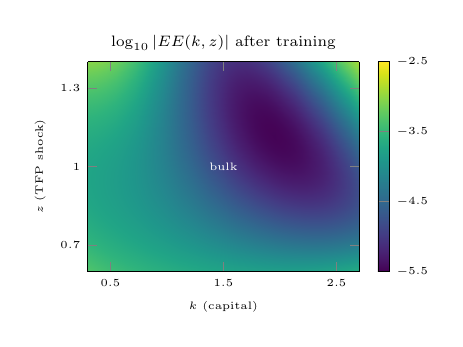
\begin{tikzpicture}[scale=0.78, transform shape]
      \begin{axis}[
        width=6.0cm, height=5.0cm,
        xlabel={$k$ (capital)}, ylabel={$z$ (TFP shock)},
        title={\scriptsize $\log_{10}|EE(k,z)|$ after training},
        title style={yshift=-0.15cm},
        xtick={0.5,1.5,2.5}, ytick={0.7,1.0,1.3},
        tick label style={font=\tiny},
        label style={font=\tiny},
        view={0}{90},
        colormap/viridis,
        colorbar,
        colorbar style={
          width=0.18cm,
          tick label style={font=\tiny},
          ytick={-5.5,-4.5,-3.5,-2.5},
        },
        point meta min=-5.5, point meta max=-2.5,
      ]
        \addplot3[
          surf, shader=interp, mesh/ordering=y varies,
          samples=30, samples y=20,
          domain=0.3:2.7, y domain=0.6:1.4,
        ] {-5 + 0.6 * ( (x-1.5)^2 + 6*(y-1)^2 ) + 0.7*sin(deg(2*x*y))};
        \node[font=\tiny,white,anchor=center] at (axis cs:1.5,1.0) {bulk};
      \end{axis}
    \end{tikzpicture}

    \vspace{-0.1cm}
    {\scriptsize\textit{The validation gate: dark = low residual (well trained); bright = boundary effects. Same shape Lab 3A/3B produces.}}
  \end{column}
\end{columns}
\end{frame}

%---------------------------------------
\begin{frame}{Comparison Against Lab 3A Ground Truth}
\begin{itemize}
  \item Analytical policy for log utility, $\delta = 1$:
    \[
      c^*(y) = (1-\alpha\beta)\, y, \qquad k'^*(y) = \alpha\beta\, y
    \]
  \medskip
  \item Validate by plotting:
    \begin{enumerate}
      \item Trained policy $g_\theta(k)$ versus $k'^*(y)$ on the same axes
      \item Pointwise error $|g_\theta(k) - k'^*(y)|$ as a function of $k$
      \item Histogram of $\log_{10}|EE(k_i)|$ across a validation sample
    \end{enumerate}
  \medskip
  \item \textbf{Sanity checks for Lab 3B (after 5{,}000 epochs)}:
    \begin{itemize}
      \item Max policy error $< 10^{-3}$
      \item Savings rate $g(k)/y$ pinned at $\alpha\beta$ across the grid
      \item Loss curve monotone-decreasing on log scale, no oscillation
    \end{itemize}
\end{itemize}
\end{frame}

%=============================================================================
% House-style bridge closer (matches Lec05/Lec09): restate the act, hand off.
\begin{frame}{Bridge: It Runs --- Now Make It Respect the Theory}
\textbf{Act 4.3 made it concrete: the Euler residual as a training loss, PolicyNet and ValueNet in PyTorch, and the training loop that drives both to the analytical solution.}

\vspace{0.25cm}
\begin{itemize}
  \item You can now code both routes to the same policy: Bellman (actor--critic) and Euler (residual minimization) --- with sanity checks against the closed form.
  \item \textbf{Next (4.4):} generic networks can violate concavity and monotonicity exactly where it hurts the solver; ICNN and monotone architectures build the theory in --- and the Lab 3A/3B audit decides whether to believe any of it.
\end{itemize}

\vspace{0.3cm}
\begin{center}
\footnotesize\textit{Arc: 4.1 PROBLEM (growth model $+$ curse) $\;\to\;$ 4.2 SOLVE (deep VFI $+$ actor--critic) $\;\to\;$ \textbf{4.3 CODE} (Euler $+$ PyTorch) $\;\to\;$ 4.4 TRUST (structure $+$ validation).}
\end{center}
\end{frame}

\end{document}
